Un variador de velocidad (VSD, por sus siglas en inglés Variable Speed Drive) es utilizado para controlar la velocidad de giro de un motor. \\
Para regular las revoluciones, se debe tener en cuenta las características del motor, ya que este tiene una curva propia de funcionamiento. Para seguir esta curva se emplea un variador pudiendo este ser utilizado junto con ventiladores, bombas, elevadores, portones, etc generando en estos elementos control de aceleración, frenado, seguridad, control del torque y operaciones que mejoran la eficiencia energética.

\subsubsection{Especificaciones}
El variador de velocidad que se utilizó pertenece a la marca \textbf{Schneider Electric} (Figura \ref{fig:variador}) que posee las siguientes características. \\
	\paragraph*{Altivar 312}
	\begin{itemize}
		\item 	Modelo: ATV312HU15N4
		\item   Tensión: 380-500 V
		\item 	Frecuencia: 50/60 Hz
		\item 	Potencia: 1.5kW / 2 HP
		\item 	Fases: 3
	\end{itemize}

	\begin{figure}[h!]
		\centering
		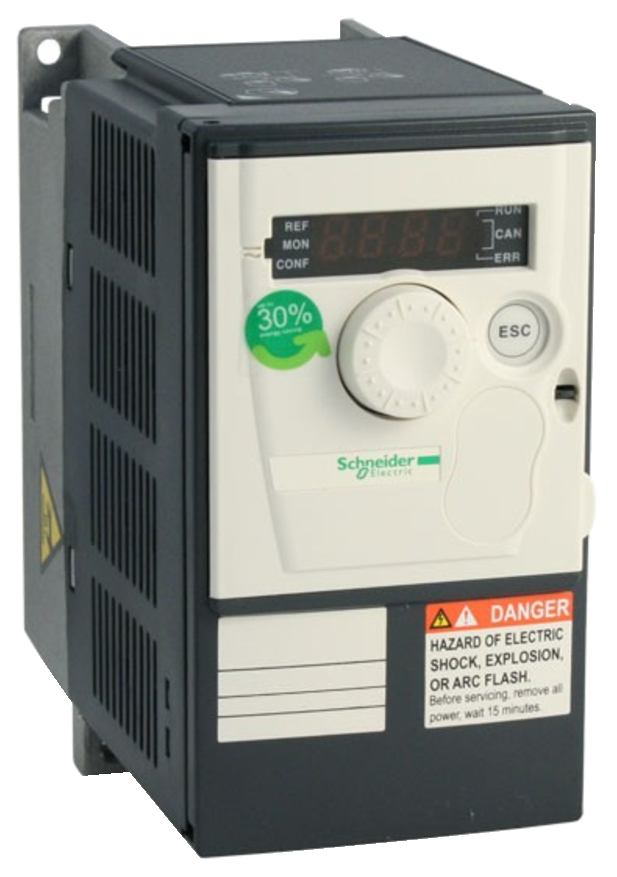
\includegraphics[scale=0.4]{variador.eps}
		\caption{Variador de velocidad Altivar 312}
		\label{fig:variador}
	\end{figure}


	\subsubsection{Configuración de parámetros primarios}
	Para realizar la configuración del motor se utilizó el software SoMove. Se descargó la ultima versión desde la página oficial de Schneider\footnote{\url{https://www.se.com/ar/es/product-range-presentation/2714-somove/}} y luego, la librería DTM correspondiente al variador a utilizar\footnote{\url{https://www.se.com/ar/es/download/document/Altivar_DTM_Library/}}. 
	\\
	Una vez realizado esto se procedió a generar un nuevo proyecto eligiendo las opciones correctas del variador.
	
	\subsubsection{Configuración de comunicación CANopen}

	\paragraph{Registros a utilizar}
	ir a ANEXO y poner la lista completa de direcciones

	\newpage

